%-*-latex-*-
This is a continuation of the \lq\lq overlapping interval problem\rq\rq from 
the previous assignment. We now want to look at overlapping
{\bf \underline{rectangles}}. A rectangle can be described by $4$ numbers.
For instance, look at the following rectangle:

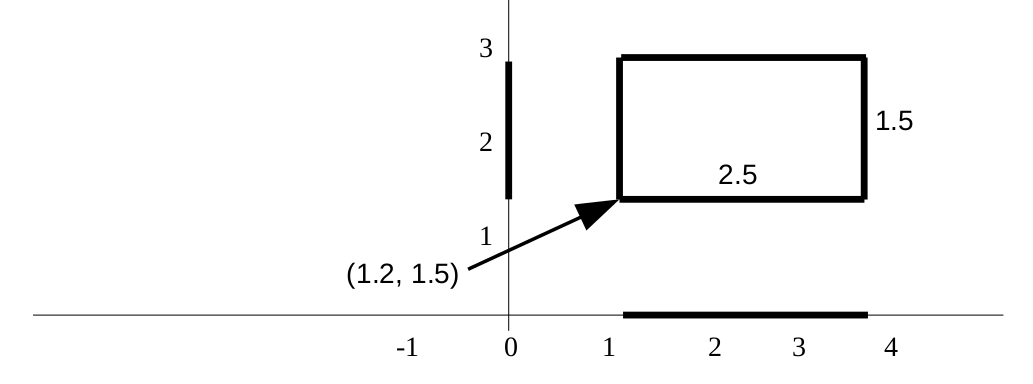
\includegraphics[width=6 in, height=2 in]{figure1.png}

The $xy$--coordinates of the lower left corner are $1.2$ and $1.5$. The width 
of the rectangle is $2.5$ while the height is $1.5$. We can therefore describe
the above rectangle with these four numbers:
\[ 1.2 \,\,\,\, 1.5 \,\,\,\, 2.5 \,\,\,\, 1.5 \]
I have also drawn the \lq\lq shadow\rq\rq of the rectangle along the $x$-- and
$y$--axis. The math folks call them projections onto the axes.

The following diagram shows two rectangles. One rectangle is from the previous 
diagram. The other is described by
\[ 3 \,\,\,\, 1 \,\,\,\, 2 \,\,\,\, 1 \]
(i.e the $xy$--coordinates 
of the lower left corner are $3$ and $1$, the width is $2$, 
and the height is $1$):

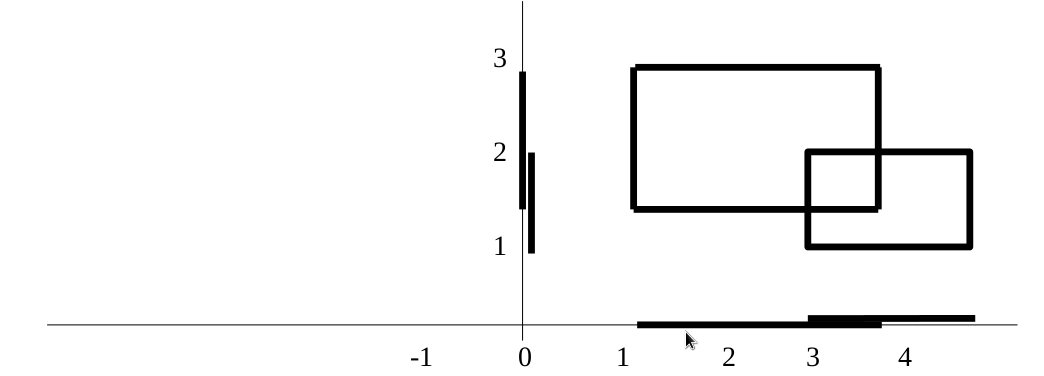
\includegraphics[width=6 in, height=2 in]{figure2.png}

Note that the two rectangles overlap. Of course there are other ways for two 
rectangles to overlap. For instance one can be \lq\lq inside\rq\rq another.

This is used in games for computing if the rectangular regions occupied by two 
images overlap. It gives an approximation of collision of two game objects:

\begin{center}

\includegraphics[width=0.5in]{figure3.png}

\includegraphics[width=0.5in]{figure4.png}
\end{center}

\begin{center}
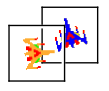
\includegraphics[width=1in]{figure5.png}
\end{center}

Write a program that prompts the user for eight numbers (doubles) where the 
first four describe one rectangle and the next four describe another. Next the 
program sets a boolean variable to true if the rectangular regions represented 
by the numbers overlap; otherwise it's set to false. Finally your program 
prints the boolean variable; i.e., the output is \verb!1! if the two intervals 
overlap, and \verb!0! if the two intervals do not overlap.

Hence, this is an execution of the program for the above scenario with the two
rectangles that overlap which will tell you that they overlap:
\begin{console}[commandchars=\\\{\}]
\userinput{1.2 1.5 2.5 1.5 3 1 2 1}
1
\end{console}

(You are encouraged to sketch some rectangles to better understand the problem.
)

\resett
\nextt
\begin{console}[commandchars=\\\{\}]
\userinput{1.2 1.5 2.5 1.5 3 1 2 1}
1
\end{console}

\nextt
\begin{console}[commandchars=\\\{\}]
\userinput{1.2 1.5 2.5 1.5 3 1 2 4}
1
\end{console}

\nextt
\begin{console}[commandchars=\\\{\}]
\userinput{1.2 1.5 2.5 1.5 0 5 2 1}
0
\end{console}

\nextt
\begin{console}[commandchars=\\\{\}]
\userinput{1.2 1.5 2.5 1.5 2 2 0.25 0.25}
1
\end{console}

\nextt
\begin{console}[commandchars=\\\{\}]
\userinput{1.2 1.5 2.5 1.5 4 1 0.25 0.25}
0
\end{console}

\nextt
\begin{console}[commandchars=\\\{\}]
\userinput{1.2 1.5 2.5 1.5 4 1 0.25 10}
0
\end{console}

\nextt
\begin{console}[commandchars=\\\{\}]
\userinput{1.2 1.5 2.5 1.5 4 1 10 0.25}
0
\end{console}

\nextt
\begin{console}[commandchars=\\\{\}]
\userinput{1.2 1.5 2.5 1.5 4 1 10 10}
0
\end{console}

\nextt
\begin{console}[commandchars=\\\{\}]
\userinput{1.2 1.5 2.5 1.5 1 1 0.25 0.25}
0
\end{console}
